% Requirements
% * Librsvg
% * Texlive-fontsextra

\documentclass[unicode]{llncs}


%% { Packages
\usepackage{xunicode}
\usepackage{xltxtra}
\usepackage[hmargin=2.5cm,vmargin=2.5cm]{geometry}
\usepackage[english]{babel}
\usepackage[babel]{csquotes}
\usepackage{url}
\usepackage{xcolor}
\usepackage[colorlinks=true,xetex]{hyperref}
\usepackage[colorinlistoftodos, textwidth=4cm, shadow]{todonotes}
\usepackage{minted}
\usepackage{import}
\usepackage{amsmath,unicode-math}
\usepackage{chngpage}
\usepackage{tabularx}
\usepackage{framed}
%% }

%% { Colors
\definecolor{Grey10}{rgb}{0.1, 0.1, 0.1}
\definecolor{Grey30}{rgb}{0.3, 0.3, 0.3}
\definecolor{Grey50}{rgb}{0.5, 0.5, 0.5}
\definecolor{Grey70}{rgb}{0.7, 0.7, 0.7}
\definecolor{Grey98}{rgb}{0.98, 0.98, 0.98}
\definecolor{Red}{rgb}{1, 0, 0}
\definecolor{Blue}{rgb}{0, 0, 1}
\definecolor{Yellow}{rgb}{0.9, 0.8, 0}
\definecolor{Purple}{rgb}{0.74, 0.2, 1}
\definecolor{LightGreen}{rgb}{0.65, 0.84, 0.52}
\definecolor{LightBlue}{rgb}{0.26, 0.75, 0.98}
%% }

%% { Fonts
\defaultfontfeatures{Ligatures=TeX} % New fonts behave like in LaTeX

\setromanfont[Mapping=tex-text]{DejaVu Serif} % Roman font
\setsansfont[Mapping=tex-text]{DejaVu Sans}  % Sans font
\setmathfont{XITS}
%% }

%% { Custom commands
%%% { To-do commands
\newcommand{\todoinline}[1]{\todo[nolist, inline]{#1}}
\newcommand{\todoaside}[1]{\todo[nolist]{#1}}

\newcommand{\codefromfile}[2]{%
  \inputminted[linenos=true, mathescape, frame=single, framesep=2mm]{#1}{#2}%
}

\newenvironment{notebox}{%
  \def\FrameCommand{\fboxsep=\FrameSep \fcolorbox{Grey10}{LightBlue}}%
  \color{Grey10}\MakeFramed {\FrameRestore}}%
 {\endMakeFramed}

%%% }
%%% { Linking commands
\newcommand{\link}[2]{\href{#1}{#2}}
%%% }
%%% { Inclusion / Import commands
% Include an SVG file converting the file into a pdf and including it
% Parameters:
%   1- the svg file path (absolute or relative to the SRC_PTH)
%   2- the image scale (from 0 to 1)
% Requirements:
%   - librsvg
\newcommand{\includesvg}[2]{%
  \immediate\write18{rsvg-convert -f pdf -o #1.pdf #1.svg}%
  \includegraphics[scale=#2]{#1.pdf}
}
%%% }
%%% { Cross-referencing commands
%%%% { Section referencing
\newcommand{\labelsec}[1]{\label{sec:#1}}
\newcommand{\xs}[1]{Section~\ref{sec:#1}}
\newcommand{\xsp}[1]{Section~\ref{sec:#1} on page~\pageref{sec:#1}}
%%%% }
%%%% { Subsection referencing
\newcommand{\labelssec}[1]{\label{ssec:#1}}
\newcommand{\xss}[1]{Subsection~\ref{ssec:#1}}
\newcommand{\xssp}[1]{Subsection~\ref{ssec:#1} on page~\pageref{ssec:#1}}
%%%% }
%%%% { Figure referencing
\newcommand{\labelfig}[1]{\label{fig:#1}}
\newcommand{\xf}[1]{Figure~\ref{fig:#1}}
\newcommand{\xfp}[1]{Figure~\ref{fig:#1} on page~\pageref{fig:#1}}
%%%% }
%%%% { Table referencing
\newcommand{\labeltab}[1]{\label{tab:#1}}
\newcommand{\xt}[1]{Table~\ref{tab:#1}}
\newcommand{\xtp}[1]{Table~\ref{tab:#1} on page~\pageref{tab:#1}}
%%%% }
%%% }
%% }


%% { Aliases
%%% { Contact informations
\newcommand{\authorname}{Alessandro Molari}
\newcommand{\authoremail}{\email{alessandro.molari@studio.unibo.it}}
\newcommand{\societyname}{Alma Mater Studiorum --- University of Bologna}
\newcommand{\addresscity}{Cesena}
\newcommand{\addresspostalcode}{47522}
\newcommand{\addressstreet}{Via Venezia 52}
\newcommand{\addresscountry}{Italy}
\newcommand{\addressfull}{%
  \addressstreet\\\addresscity, \addresspostalcode\\\addresscountry%
}
%%% }
%%% { Shortcuts
\newcommand{\gaugesystem}{\texttt{Gauge System}}
\newcommand{\mdsd}{\link{http://en.wikipedia.org/wiki/Model-driven_architecture}{\texttt{MDSD}}}
\newcommand{\umlclassdiagram}{\link{http://www.agilemodeling.com/artifacts/classDiagram.htm}{\texttt{UML v2.3} Class diagram}}
\newcommand{\mindmap}{\link{http://en.wikipedia.org/wiki/Mind_map}{MindMap}}
\newcommand{\iterativeprocess}{\link{http://c2.com/cgi/wiki?IterativeDevelopment}{Iterative Process}}
\newcommand{\junit}{\link{http://www.junit.org}{\texttt{jUnit v4}}}
\newcommand{\abstracttest}{\link{http://c2.com/cgi/wiki?UnitTestingAbstractBaseClasses}{\texttt{Unit Testing Abstract Base Classes}}}
\newcommand{\java}{\link{http://openjdk.java.net}{Java}}
\newcommand{\principlepareto}{\link{http://en.wikipedia.org/wiki/Pareto_principle}{80/20 Principle}}
\newcommand{\scm}{\link{http://en.wikipedia.org/wiki/Revision_control}{\texttt{SCM}}}
\newcommand{\cpm}{\link{http://en.wikipedia.org/wiki/Critical_path_method}{\texttt{CPM}}}
\newcommand{\cmm}{\link{http://en.wikipedia.org/wiki/Capability_Maturity_Model}{\texttt{CMM}}}
\newcommand{\pmt}{\link{http://en.wikipedia.org/wiki/Project_management_triangle}{\texttt{Project Management Triangle}}}
\newcommand{\designpatterns}{\link{http://www.oodesign.com}{\texttt{Design Patterns}}}
%%% }
%% }


\author{\authorname}
\title{Distributed Middleware Overview}
\institute{\societyname\\\addressfull\\\authoremail}

\begin{document}

  \maketitle
  \clearpage

  %%% =80 chars================================================================
  \section{The fundamental idea}
  \labelsec{FundamentalIdea}

    \begin{figure}[H]
      \centering
      \includegraphics{resources/CommunicationModel.png}
      \caption{Communication Model}
    \end{figure}

    \begin{figure}[H]
      \centering
      \includegraphics{resources/Layers.png}
      \caption{Layers}
    \end{figure}

    \begin{figure}[H]
      \centering
      \includegraphics{resources/ConceptualView.png}
      \caption{Conceptual View}
    \end{figure}

  \section{Half-duplex vs Full-duplex}
  \labelsec{HalfFullDuplex}

    When we designed the middleware we had choose between two alternatives:
    \begin{itemize}
      \item \textbf{Native full-duplex communication}:
        An entity that interfaces itself with the communication channel
        must be able to both send and receive.
      \item \textbf{Native half-duplex communication}:
        An entity that interfaces itself with the communication channel can
        send or receive, but it \textit{doesn't have} to be able to do both
        of them.
    \end{itemize}
    The first alternative is \textbf{unflexible} because an entity that wants
    to send and receive in the channel (i.e. wants some feedback about the
    sent data) from the communication cannot do that.\newline
    In addition, with the first alternative the
    \textbf{parameters of the communication} (like \textit{QoS},
    \textit{Security}) cannot be different in the two communication sides.\newline
    Last but not least, the first alternative implies that if an object in our
    system needs to communicate with another, it has to be able to both
    send or receive. We generally don't want that: an entity may want to only
    send or only receive. The problem is that there is no separation of concerns
    between the communication interface of the entities and the their
    business-logic.
    To solve this problem we could say: "Ok. An object in the system basically
    is not able to communicate with another, but if he implements the sending
    interface he can send and if he wants to receive he can receive". These
    interfaces in the system are called \texttt{ObservableEndpoint} and
    \texttt{ObserverEndpoint}.

    Now that we have chosen to separate the interfaces of sending and receiving
    we ask ourself:\newline
    "We found some disadvantages for the first alternative. What are the
    advantages of a native full-duplex communication?".\newline
    The answer that we found is: "None because with a middleware the
    first alternative is unhelpful and valueless".

    The second alternative is a lot more flexible because it can act as
    a full-duplex communication between the entities if they implement
    both of the interfaces (\texttt{ObservableEndpoint} and
    \texttt{ObserverEndpoint}).\newline
    In addition if we want to use a channel for both sides we can: we just need
    that each endpoint sends and receives from the same channel.
    If we want different communication channels for the two communication sides
    we can: we create two half-duplex channels.

    \begin{figure}[H]
      \centering
      \includegraphics{resources/FullDuplexCommunication.png}
      \caption{Photo of the author}
    \end{figure}

  \section{Structure}
  \labelsec{Structure}

    This is the structure of the middleware:
    \begin{figure}[H]
      \centering
      \advance\leftskip-1cm
      \def\svgwidth{\columnwidth}
      \includesvg{resources/StructureMiddleware}{0.2}
      \caption{Structure}
    \end{figure}

  \section{Interaction}
  \labelsec{Interaction}

    The interaction model has been divided in three submodels:
    \begin{itemize}
      \item Local communication: The \texttt{ObservableEndpoint} and
        the \texttt{ObserverEndpoint} are in the same context.
      \item Remote communication
        \begin{itemize}
          \item Iteractions for the sender
          \item Iteractions for the receiver
        \end{itemize}
    \end{itemize}

    \begin{figure}[H]
      \centering
      \advance\leftskip-1cm
      \def\svgwidth{\columnwidth}
      \includesvg{resources/InteractionLocalSenderReceiver}{0.2}
      \caption{Interaction - Local sender / Local receiver}
    \end{figure}

    \begin{figure}[H]
      \centering
      \advance\leftskip-1cm
      \def\svgwidth{\columnwidth}
      \includesvg{resources/InteractionRemoteReceiver}{0.2}
      \caption{Interaction - Remote receiver}
    \end{figure}

    \begin{figure}[H]
      \centering
      \advance\leftskip-1cm
      \def\svgwidth{\columnwidth}
      \includesvg{resources/InteractionRemoteSender}{0.4}
      \caption{Interaction - Remote sender}
    \end{figure}

        L'idea di fondo e' che in un sistema esistano entita' che vogliano comunicare
    fra di loro tramite un mezzo di comunicazione condiviso.
    Un requisito fondamentale e' che tali entita' comunichino in maniera disaccoppiata
    tramite un opportuno middleware di comunicazione.\cite{gof94}


    Tali entita' possono comunicare in un ambiente concentrato oppure distribuito,
    ma certamente tali entita' non vogliono conoscere le problematiche di comunicazione.
    In realta' non vogliono neanche conoscere se la comunicazione avverra' in maniera
    locale oppure distribuita. Inoltre per garantire flessibilita' al sistema e' necessario
    un modello di comunicazione in cui le entita' non si conoscano fra di loro.
    In realta' un'entita' che invia non sa neanche chi/se ci sara' a ricevere il messaggio:
    il suo unico compito e' inviare, niente di piu'. Allo stesso modo il ricevitore semplicemente
    e' interessato a ricevere token dal middleware, mentre e' completamente disinteressato
    alla comunicazione che e' avvenuta per far pervenire tali tokens a lui.

' Interaction between the gauges and the displays through the middleware.
' In this interaction model the gauges don't know anything about the
' receivers (they could be displays or anything that is subscribed in the
' middleware).
' The gauges only talk with the sender-side of the middleware.
' The displays only talk with the receiver-side of the middleware.
' The middleware is half-duplex. This empowers flexibility when doing
' full-duplex communication by separating the policies for both sides of the
' communication. In this case it's used in half-duplex because the gauges don't
' want any feedback from the messages receivers.
' Here we explain the two-tier interaction but the flexibility and the power
' of this middleware makes the choice about two-tier vs three-tier only a matter
' of configuration.
' Theoretically (and practically) that choice could be make at runtime, maybe
' based on the status of the environment!

  %%% =80 chars================================================================
  \section{Information about the author}
  \labelsec{Author}

    \begin{itemize}
      \item Full Name: \authorname
      \item Code: 0000490818
      \item Email: \authoremail
    \end{itemize}
    \begin{figure}[H]
      \centering
      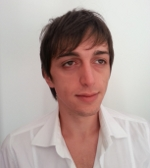
\includegraphics[scale=0.7]{resources/authorphoto.png}
      \caption{Photo of the author}
    \end{figure}

  %%% =80 chars================================================================
  \appendix

  % The list of the used references
  \clearpage
  \bibliographystyle{abbrv}
  \bibliography{biblio}

  % The Table of Contents
  \clearpage
  \setcounter{tocdepth}{4}
  \tableofcontents
\end{document}

% vim: filetype=tex:

